\chapter{Roots}\label{chap:roots}

In the traditional way of learning, to know a verb means to know its root. So, it is really important to identify a root when we encounter a verb. Learning Pāli roots, unfortunately, is not an easy task because different schools name roots differently. Furthermore, some roots can behave strangely in certain contexts. So, in modern way of learning Pāli, knowing roots is less pressing.\footnote{It is easier to learn verbs by its \pali{-ti} form, which gives us its stem, not root.} But knowing them still brings great benefits.

Roots listed here come from the compilation of Ven.\ U Silana\-nda in \emph{Pali Roots in Saddanīti Dhātu-Mālā compared with Pāṇinīya-Dhātupāṭha}.\footnote{Edited by U Nandisena, \url{archive.org/details/ThePaliRootsInSaddaniti}} So, the roots are familiar to those who follow Kaccāyana/Saddanīti school.

Things the users can do with the roots are: you can select only a specific verb group; you can search in the roots' name, in Pāli meaning, and in English meaning. Figure \ref{fig:roots} show Roots window with an option opened.

\begin{figure}[!hbt]
\centering
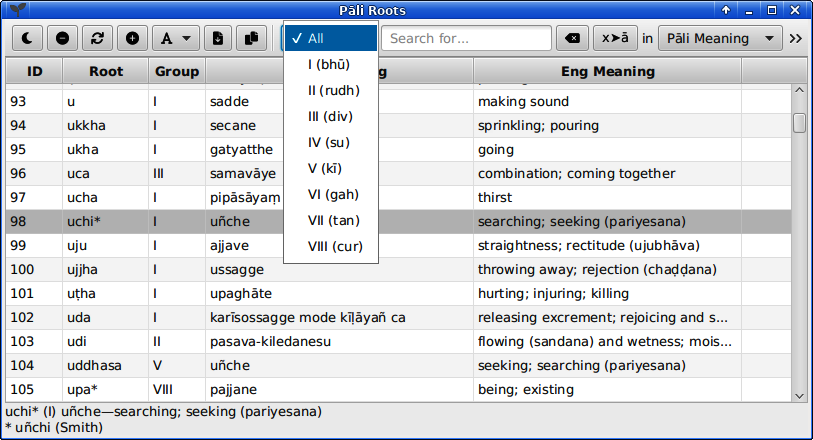
\includegraphics[width=0.9\linewidth]{images/roots.png}\\
\caption{Roots window}
\label{fig:roots}
\end{figure}

In some entries, you can see an asterisk (*) mark in the root's name. In some, you can also see double asterisks (**) in the Pāli meaning. These marks tell us that there is a comment in the entry. You can see the comment by clicking the row in the table. Comments are directly taken from the original work. So, some of them can be difficult to understand exactly.\footnote{\emph{Smith} mentioned by comments is the publication of Saddanīti edited by H.\ Smith (1928--66), 6 volumes. In this context it means the second volume (Dhātumālā) of that work. The 5 volumes of the first edition can be found at \url{archive.org/details/SaddanitiAggavamsasPaliGrammar01} (to 05).}

The best way to study these roots, I suggest, is by reading Saddanīti Dhātumālā (available in the collection of traditional grammar books) directly on the root you are interested in. In addition, DPD also has its root list, which uses more generic names. It is a good idea to check against that list as well. 

Furthermore, as a new tool, {\faSix \symbol{"F002}} Pāli Root Finder gives you the most exhaustive list of roots (see Chapter \ref{chap:rootfinder}).

